\subsection{Second Order Effects} \label{subsection:second_order_effects}

In the derivation of the current-voltage characteristics of the MOSFET, we
assumed that certain properties are constant under all operating conditions. These ideal assumptions do not apply in a real device. Some examples of the non-idealities in a MOSFET are described here.  

\subsubsection{Prelude: How transistor width and length impact operation}

Remember that both the sub- and the superthreshold current are scaled by a parameterized factor: $I_0$ and $\beta$ where

\begin{equation}
    I_0 = q \frac{W}{L} t D_n N_0 e^{\frac{-\phi_0}{U_T}}
\end{equation}

\begin{equation}
    \beta = \mu C_{ox} \frac{W}{L}
\end{equation}

Both factors are dependent on the ratio between the transistor's width and its length $\frac{W}{L}$. This is an important condition to consider when designing MOSFETs. Simply looking at this condition, it seems desirable to keep our transistor length as small as possible in order to get a power efficient transistor. In reality, the length of the channel defines the impact of second order effects onto our generated current flow and it is typically desired to have a longer channel. An ideal width to length ratio is therefore a very tricky design decision. The following sections will introduce the most important second order effects and in particular how they are shaped by the transistor's length.

\subsubsection{Transistors in real life, and the problem of mismatch}\label{sec:device_mismatch}

You may have heard of Moore's law?\footnote{Moore's law was actually a term coined by Carver Mead!}. The observation is named after Gordon Moore, the co-founder of Fairchild Semiconductor and Intel (and former CEO of the latter), who in 1965 posited a doubling every year in the number of components per integrated circuit. The fundamental component of the integrated circuit is the transistor - so this implies that transistor are supposed to halve in size every year! Due to extremely fancy industrial processes, the smallest transistors today are as small as a few nanometers length (length from source to drain). We're now reaching the physical limits of Moore's law as the transistor has a theoretical minimum length, and it wouldn't function the same way if we ever manage to make it smaller. Besides this issue, we should note something: transistor function is impacted by their sizes. There are many \textit{second order effects} that are typically omitted in the modelling because they are negligible, however, because we're dealing with the limitation of the physics, these second order effects become important. We'll look at these in more details in the next chapter, but what I'd like you to remember is the fact that a difference in size of 1 mm between two Ikea shelves will not matter when you build your piece of furniture, because 1mm is negligible compared to the overall size of the shelf. However, if you have a 1cm difference, it might start to be a problem. Similarly with the transistor, because we're dealing with extremely small components, and because the industrial processes cannot realistically be precise to the $10^{-12}$, you always end up with slight size differences between the transistors within a circuit, which lead to some differences in the way they function, and is the source of many limitations in modern VLSI. This problem is name \textbf{transistor mismatch} and it is going to appear very often in your lab plots, as you will see when you start experimenting with the Class Chip.

\subsubsection{The Early Effect}

Very, very important thing to start with: it's named after James Early, and is not related to being early, late or anything time related. I wanted to mention it first because to this day I unconsciously picture it as something happening before something else. 
The lecture notes state: "When deriving the I-V (Current-Voltage) characteristics of nFETs in the previous chapter, we assumed that the current is constant when working in saturation ($V_{ds} > 4U_T$). It so happens that this assumption is not sufficient, especially with short length MOSFETs, for which the drain voltage can modulate the channel current, even in saturation." So what is exactly happening here?  
Let's start by reminding ourselves the (nFET) relationship and the theoretical graph linking drain current $I_{ds}$ to drain to source voltage $V_{ds}$ for fixed $V_{gs}$:

\begin{equation}
I_{ds} = I_{n0} e^{\frac{\kappa_{n}V_g}{U_T}}(e^\frac{-V_s}{U_T} - e^\frac{-V_d}{U_T})
\end{equation}

We also should look at the graphical relationship this relation implies:

\begin{figure}[H]
    \centering
    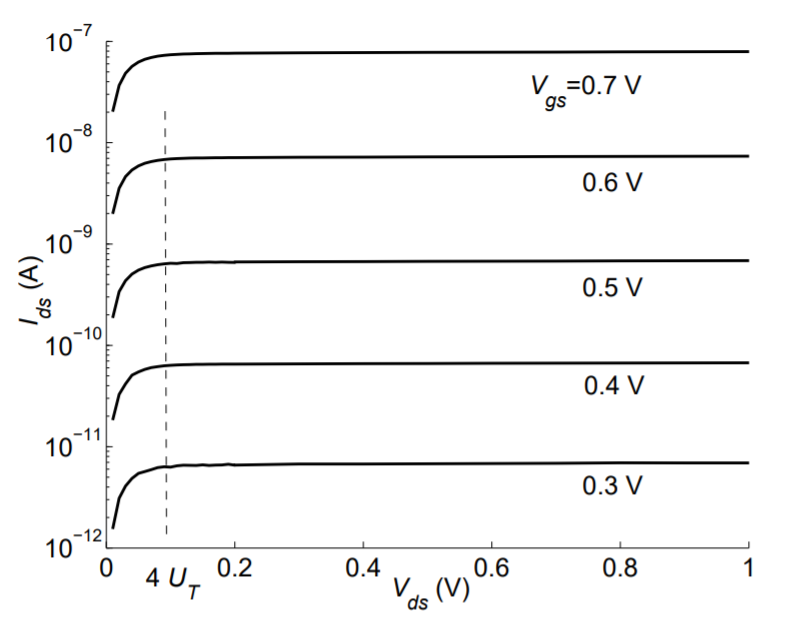
\includegraphics[width=0.7\linewidth]{../../Figures/Vds_Vs_Ids_No_Early_Effect.PNG}
    \caption{Relationship between $V_{ds}$ and $I_{ds}$ for fixed $V_{gs}$. Determines the voltage at which we switch from Ohmic to Saturation region. Adapted from Lecture Notes.}
    \label{fig:vdsids}
\end{figure}

One should notice in the equation and that $I_{ds}$ has an almost insignificant dependence on $V_{ds}$, because of the exponential term, where the term in parenthesis just vanishes to $V_{s}$ as $V_{d}$ (and thus $V_{ds}$) increases. We consider this to start being true when $V_{ds} > 4U_T$, where we go from the "Ohmic" Region to the "Saturation region". This is clearly apparent in figure \ref{fig:vdsids}, where changing $V_{ds}$ does not affect $I_{ds}$ past the 4$U_T$ threshold - thus yielding a constant relationship between $V_{ds}$ and $I_{ds}$ past the threshold (again, taking $V_{gs}$ as fixed). 

Now surprise surprise, this model is not correct in practice. This is called the Early effect, and basically introduces the practical problem of slightly rising $I_{ds}$ when increasing $V_{ds}$, even past the the saturation threshold. This rate of change is critically impacted by the geometry of the transistor, mainly its W/L ratio. Effectively, when increasing $V_d$, the \emph{effective length $L_{eff}$} of the transistor decreases. This is because the pinchoff region extends further along the channel away from the drain (see figure below). This has a particularly important impact when we are dealing with short transistors, as the shift in pinchoff is, relatively to the channel length, more important (see figure \ref{fig:pinchoff}). 

\begin{figure}[H]
    \centering
    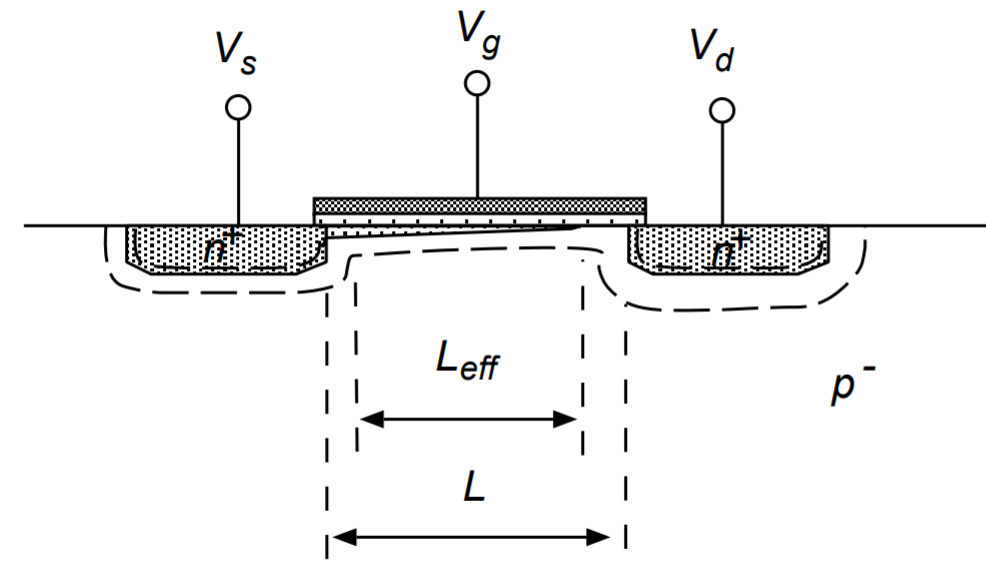
\includegraphics[width=0.7\linewidth]{../../Figures/Early_Effect_Pinchoff_Region.PNG}
    \caption{The effective channel length $L_{eff}$ of a transistor operating in the above-threshold saturation region decreases with increasing Vd because the pinchoff point moves into the channel, away from the drain. The effective channel length can be described by the transistor length minus the length of the pinchoff region in the channel. Adapted from Lecture Notes.}
    \label{fig:pinchoff}
\end{figure}

Ok great. So what do we do with this information? Well now we need to find a way to quantify this effect and include it in the previous equation to have a more accurate model. For this, we need to use the \emph{Early Voltage} and the following relations: 

\begin{figure}[H]
    \centering
    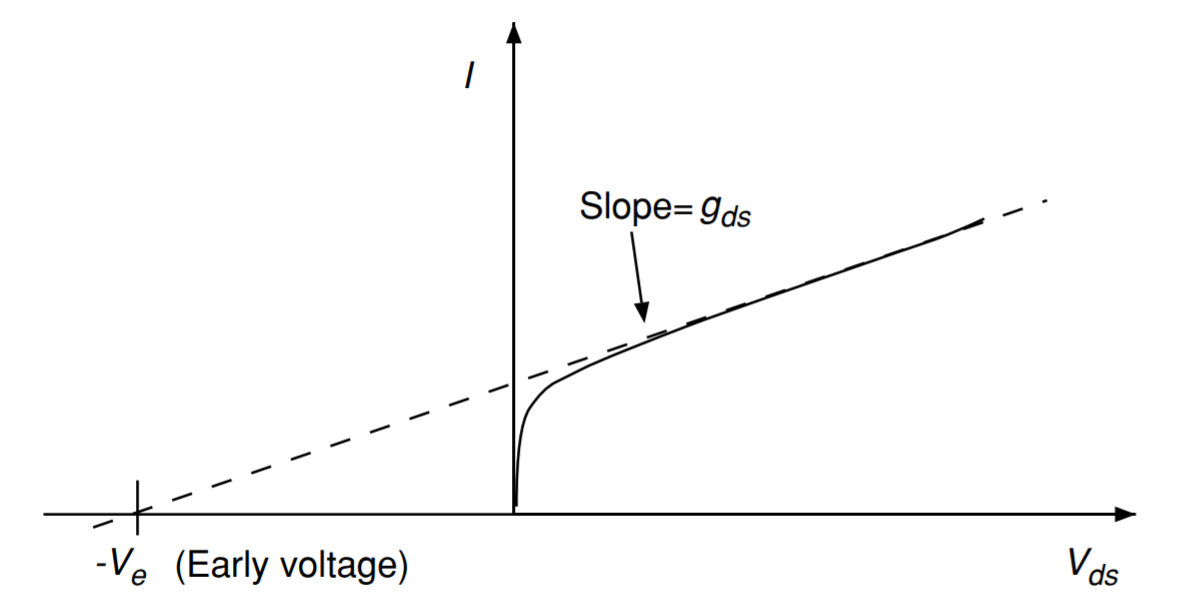
\includegraphics[width=0.7\linewidth]{../../Figures/Early_Voltage.PNG}
    \caption{Plot of current versus drain-to-source voltage, showing the slope of the curve gds in the saturation regime. The intersection of the slope with the Vds axis is called the Early voltage. Adapted from Lecture Notes.}
    \label{fig:basalandcerebellum}
\end{figure}

We just established that even in Saturation, there is a slight increase in $I_{ds}$ as a function of increasing $V_{d}$ - this increase is linear as shown in the figure above, and it has a very specific slope called $g_{ds}$, also called the \emph{output conductance} of the transistor. It is defined as follows: 

\begin{equation}
g_{ds} = \frac{\partial I}{\partial V_{ds}} = \frac{\partial I}{\partial L_{eff}}\frac{\partial L_{eff}}{\partial V_{ds}} = \frac{I}{V_e} \label{eq:early_effect}
\end{equation}

$V_{e}$ is the \emph{Early Voltage}, which is defined as the \textbf{absolute value of voltage for which $I_{ds}$ is 0} when in saturation. \textbf{It is only a theoretical voltage that allows you to quantify the steepness of the $I_{ds}$ slope in saturation, and thus the extent by which $I_{ds}$ changes as a function of $V_{ds}$ changes.}
Understanding the precise derivation of the equation requires a substantial amount of device physics, which is out of the scope of these lecture notes. If you would like to understand better, refer to the Textbook, Chapter 3. Now accepting equation \ref{eq:early_effect} as true, we can rewrite our equation for drain current in a more complete manner, as follows:

\begin{equation}
    I = I_{sat} + g_{ds}V_{ds} = I_{sat}(1 + \frac{V_{ds}}{V_e})
\end{equation}

Here, $I_{sat}$ =  $I_{n0} e^{\frac{\kappa_{n}V_g - V_s}{U_T}}$
Should you really care about this second order effect? Yes, because $V_E$ ranges between 750V and 20V for typical transistors operating in Subthreshold, as shown in the figure below: 

\begin{figure}[H]
    \centering
    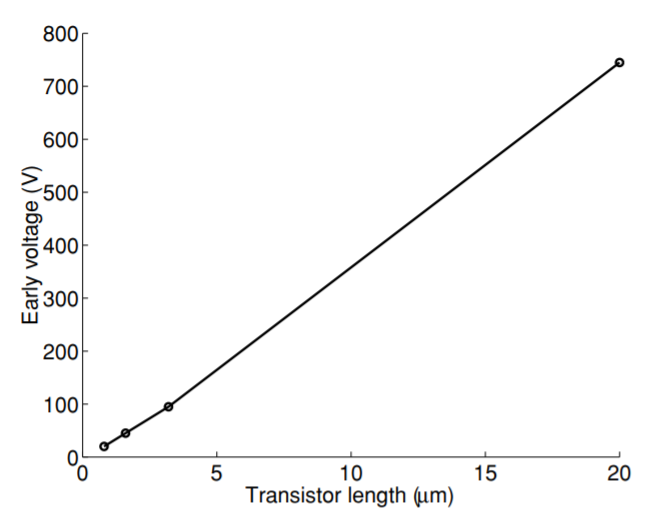
\includegraphics[width=0.65\linewidth]{../../Figures/Early_Voltage_Vs_MOSFET_Length.PNG}
    \caption{Early voltage versus the transistor length of an nFET fabricated in a 0.8 $\mu m$ CMOS proces. Adapted from Lecture Notes.}
    \label{fig:basalandcerebellum}
\end{figure}

Keep in mind that 20V is a way more significant Early Voltage than 750V, because that equates to a lot steeper slope! This is why Early Voltage is particularly important in shorter MOSFETs: a slight change in $V_{ds}$ will have significant impact on $I_{ds}$ when in Saturation! The smaller the transistor, the smaller $V_E$, and the smaller $V_E$, the higher $\frac{\partial I}{\partial V_{ds}}$. 

\subsubsection{The Body Effect}\label{sec:body_effect}

The \textit{Body Effect}, also called the \textit{Back Gate Effect} relates to the bulk and its influence on transistor operation. In the I-V (Current to Voltage) equations that we have derived so far, the terminal voltages of
the transistor are referenced to the bulk. However, the bulk is also an input to the transistor that should be considered in most circumstances, though we often chose to neglect it for simplicity.  In the subthreshold region, we can describe the influence of the bulk potential $V_b$ through the series of capacitors $C_{ox}$ and $C_d$ (as we saw also for the gate input).
The effect on the surface potential can be written as: 

\begin{equation}
    \partial \psi_s = (1-\kappa)\partial{V_b}
\end{equation}

In the strong inversion, or above-threshold, regime the influence of the
bulk voltage is usually treated as an increase in the threshold voltage of the
transistor. If $V_b$ decreases, then there is practically no change in the gate charge because the voltage across the gate oxide is essentially unchanged (the surface potential remains approximately the same). However, the depletion region underneath the gate increases \footnote{Remember from the PN Junction that increasing the reverse bias across a PN junction causes the depletion to increase}. Since the negative charge from the depletion region is now larger, less charge is required in the inversion region to balance the gate charge. The inversion region becomes smaller, so leading to a smaller $I$. To restore $I$ to its original value, we increase the gate voltage $V_{gs}$. Assuming that we do not forward the PN junctions between the drain/source regions and the bulk: What happens if the bulk voltage $V_b$ is increased by $\Delta V$?
This scenario is the same as decreasing $V_g , V_s, and V_d$ by the same $\Delta V$. In the subthreshold region, the change in $\psi_s$ will now be $-\kappa \Delta V$ . The barrier height is decreased at both ends of the channel, and the current increases. Hence, the bulk acts like the gate, but it has a weaker influence on the transistor current.

\subsubsection{Drain Induced Barrier Lowering (DIBL)}\label{sec:dibl}

In the weak inversion regime there is a potential barrier between the source and the channel region. The height of this barrier is a result of the balance between drift and diffusion current between these two regions. If a high drain voltage is applied, the barrier height can decrease, as indicated in figure \ref{fig:dibl3}, leading to an increase in the surface potential \ref{fig:dibl1}, which then also leads to an increased drain current as shown in figure \ref{fig:dibl2}. The precise derivation of this barrier lowering effect is more complicated and not part of this course, you just have to know, that it exists.\\

\begin{figure}[H]
    \centering
    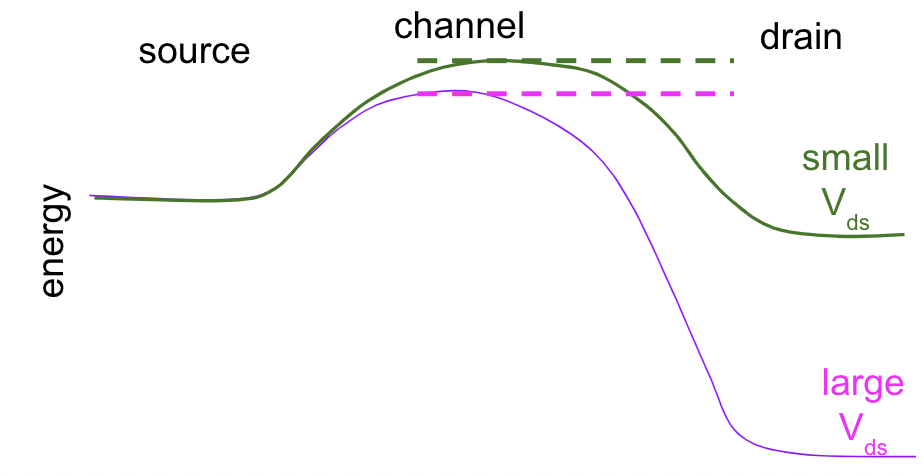
\includegraphics[width=0.65\linewidth]{../../Figures/dibl3.png}
    \caption{Varying energy barrier for different drain voltages due to Drain Induced Barrier Lowering (DIBL).}
    \label{fig:dibl3}
\end{figure}

To summarize, Drain Induced Barrier Lowering means, that the drain current is controlled not only by the gate voltage, but also by the drain voltage (although rather weakly), because a higher drain voltage decreases the energy barrier between source and channel. It is especially pronounced in small width transistors, as there the drain can influence the source more easily. Since this parasitic effect simply shifts the current up or down, it can be accounted for by a threshold voltage reduction depending on the drain voltage for device modeling purposes. Large drain voltages typically decrease the threshold voltage $V_thr$ by $\approx 100mV$. 

\begin{figure}
\centering
\begin{subfigure}{0.5\textwidth}
  \centering
  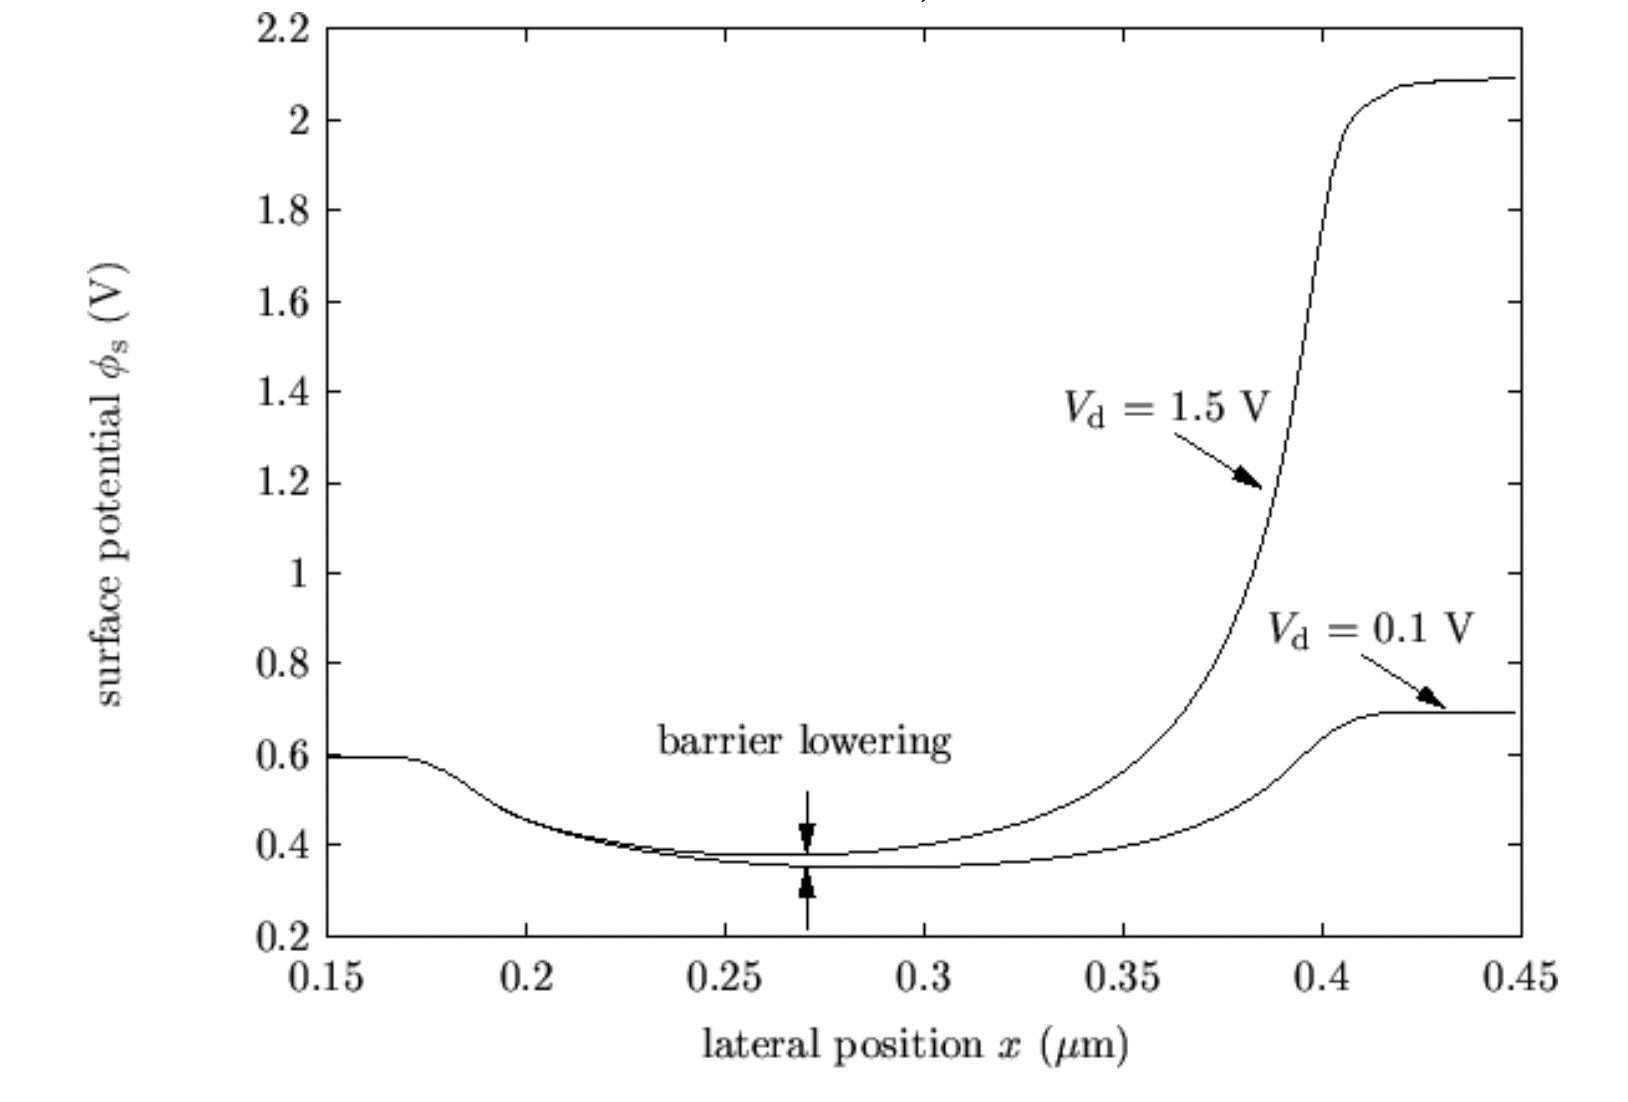
\includegraphics[width=\linewidth]{../../Figures/dibl1.png}
    \label{fig:dibl1}
\end{subfigure}%
\begin{subfigure}{0.5\textwidth}
  \centering
  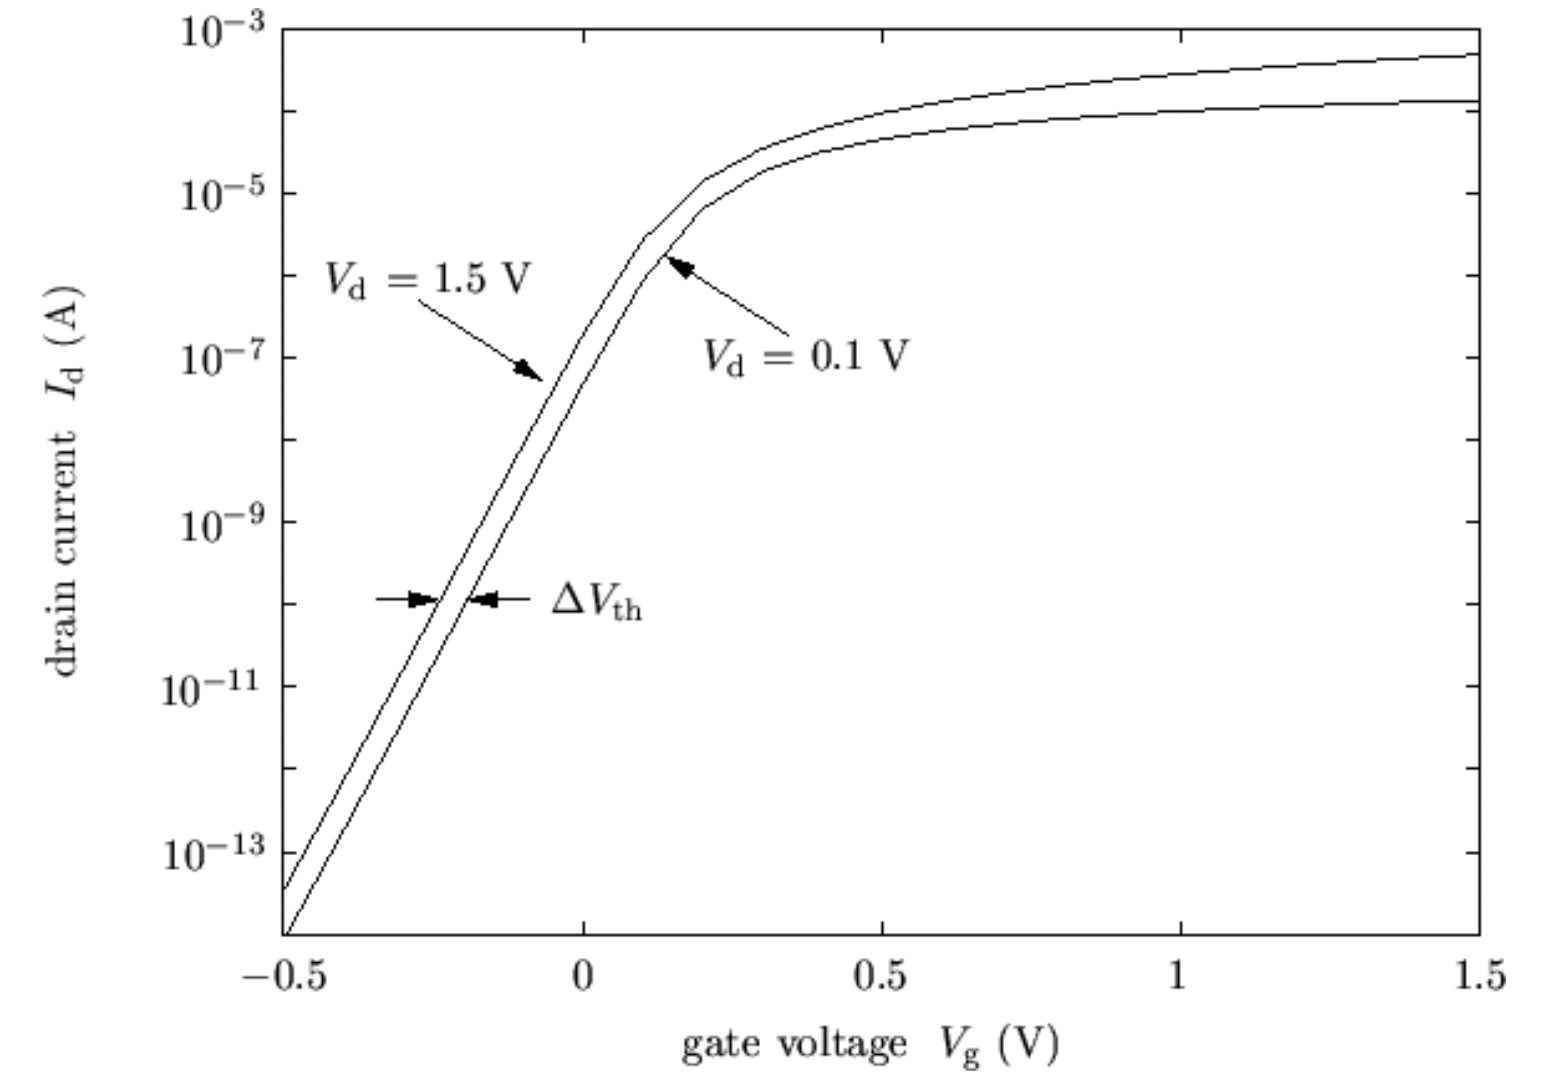
\includegraphics[width=\linewidth]{../../Figures/dibl2.png}
    \label{fig:dibl2}
\end{subfigure}
\caption{Varying surface potentials (left) and I-V curve (right) for different drain voltages due to Drain Induced Barrier Lowering (DIBL).}
\end{figure}

\subsection{Impact Ionization}

Finally, large drain voltages can lead to another effect called Impact Ionization. This simply means, that when the drain voltage is very high, it can give the incoming electrons enough kinetic energy, such that, when they bump into other bound electrons (in the valency band), the impact transfers enough energy to free them and elevate them into the conduction band, which leaves a free hole in the valency band, thus creating a new energy-hole pair (figure \ref{fig:impactIonisation2}). You can picture this as the drain acting similar to a vacuum cleaner that sucks the electrons in and the higher the voltage, the higher the power of the vacuum cleaner and the faster the electrons get sucked in hence the more kinetic energy they have and if they have enough energy they knock the bound electrons out of their bound state upon impact. The newly created electrons are naturally also affected by the drain voltage and hence also sucked in. As a result, the drain current becomes even larger than the source current (as seen in figure \ref{fig:impactIonisation2}.\\

\begin{figure}[H]
    \centering
    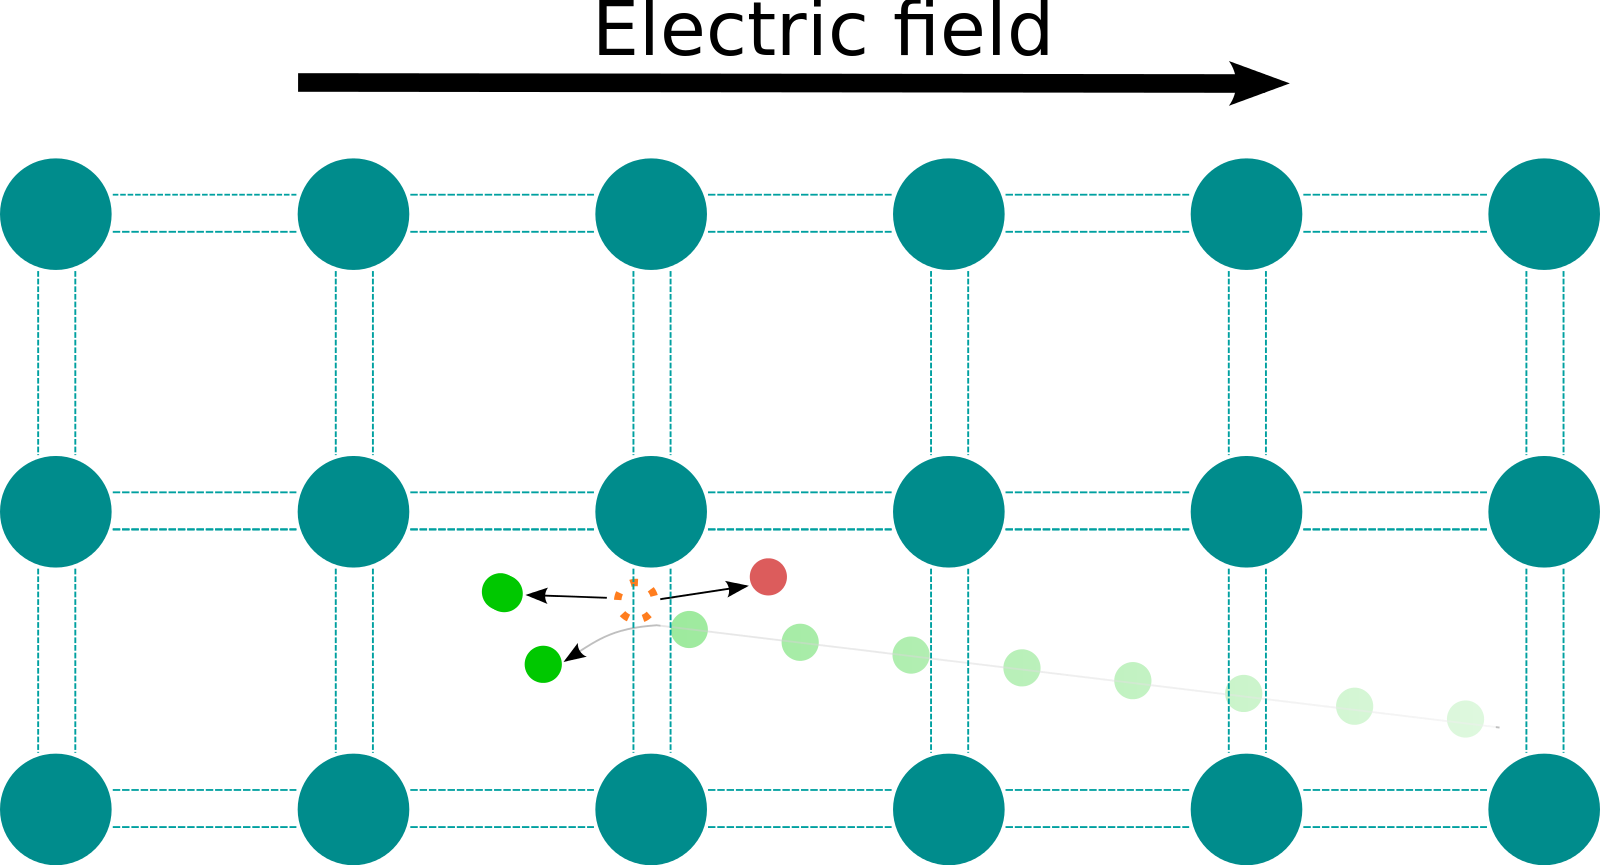
\includegraphics[width=0.65\linewidth]{../../Figures/ImpactIonisation1.png}
    \caption{}
    \label{fig:impactIonisation}
\end{figure}

We do not go into detail of the above mentioned drain effects (DIBL and Impact Ionization) but it is important to know that our derived equations neglect several phenomenons that occur in real transistors.\\

\begin{figure}[H]
    \centering
    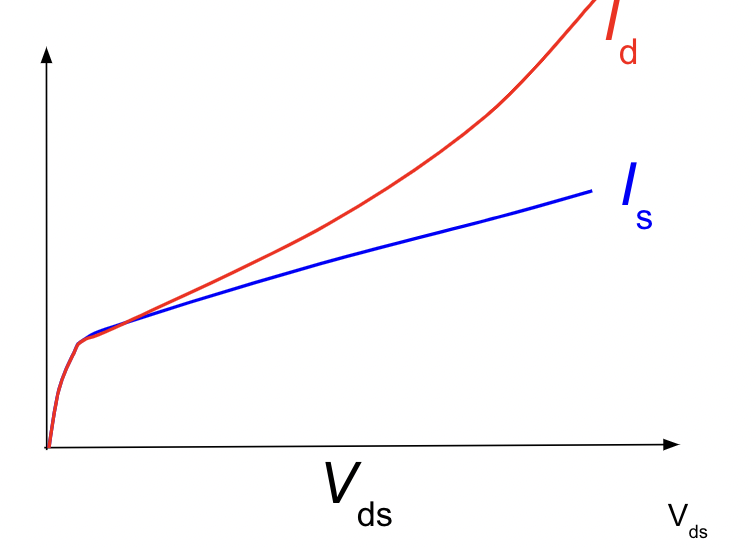
\includegraphics[width=0.65\linewidth]{../../Figures/ImpactIonisation2.png}
    \caption{}
    \label{fig:impactIonisation2}
\end{figure}